% (c) 2012 -2014 Dimitrios Vrettos - d.vrettos@gmail.com
% (c) 2014 Daniele Zambelli - daniele.zambelli@gmail.com

\chapter{Insiemi}

\section{Definizioni}
\label{sec:insiemi_definizioni}

In matematica usiamo la parola \textit{insieme} per indicare un
raggruppamento, una collezione, una raccolta di oggetti, individui,
simboli, numeri, figure che sono detti \textit{elementi}
dell'insieme e che sono ben definiti e distinti tra di
loro.

\subsection{Elementi primitivi della teoria degli insiemi}
\label{subsec:el_prim}

La nozione di insieme e quella di elemento di un insieme in matematica
sono considerate nozioni primitive, nozioni che si preferisce non
definire mediante altre più semplici.

\begin{exrig}
 \begin{esempio}
 Sono insiemi:
 \begin{enumeratea}
  \item l'insieme delle lettere della parola RUOTA;
  \item l'insieme delle canzoni che ho ascoltato la settimana scorsa;
  \item l'insieme delle città della Puglia con più di~15\,000 abitanti;
  \item l'insieme delle lettere dell'alfabeto italiano;
  \item l'insieme dei numeri~1, 2, 3, 4, 5;
  \item l'insieme delle montagne d'Italia più alte di~1\,000 metri.
 \end{enumeratea}
 \end{esempio}
\end{exrig}

Per poter assegnare un insieme occorre soddisfare le seguenti condizioni:

\begin{itemize*}
\item bisogna poter stabilire con certezza e oggettività se un oggetto
è o non è un elemento dell'insieme;
\item gli elementi di uno stesso insieme devono essere differenti tra
loro, cioè un elemento non può essere ripetuto nello stesso insieme.
\end{itemize*}

Non possono essere considerati insiemi:
\begin{itemize*}
 \item i film interessanti (non c'è un criterio oggettivo per stabilire se un 
 film è interessante oppure no, uno stesso film
 può risultare interessante per alcune persone e non interessante per altre);
 \item le ragazze simpatiche di una classe (non possiamo stabilire in maniera 
 oggettiva se una ragazza è simpatica);
 \item le montagne più alte d'Italia (non possiamo dire se una montagna è tra 
 le più alte poiché non è fissata un'altezza limite);
 \item l'insieme delle grandi città d'Europa (non c'è un criterio per
stabilire se una città è grande);
\end{itemize*}

% \ovalbox{\risolvi \ref{ese:5.1}}\vspazio

In generale, gli insiemi si indicano con lettere maiuscole~$A, B, C\ldots$
gli elementi con lettere minuscole~$a, b, c\ldots$.
Se un elemento~$a$ sta nell'insieme~$A$ si scrive~$a\in A$ e si legge 
``$a$ appartiene ad~$A$''.
Il simbolo ``$\in$'' si chiama simbolo di \textit{appartenenza}.

Se un elemento~$b$ non sta nell'insieme~$A$ si dice
che esso non appartiene all'insieme, si scrive~$b\notin A$,
si legge ``$b$ non appartiene ad~$A$''. Il simbolo ''$\notin$''
si chiama simbolo di \textit{non appartenenza}.

Il criterio che stabilisce se un elemento appartiene a un insieme si chiama 
\textit{proprietà caratteristica}.

Gli elementi di un insieme si elencano separati dalla virgola e racchiusi tra 
parentesi graffe:~$A=\{a,b,c,d\}$.

Alcuni simboli sono utilizzati per indicare alcuni insiemi specifici:
\begin{itemize*}
 \item $\insN$ si utilizza per indicare l'insieme dei numeri 
  naturali:~$\insN=\{0,1,2,3,\ldots\}$
 \item $\insZ$ si utilizza per indicare i numeri interi 
  relativi:~$Z=\{\ldots,-3,-2,-1,0,+1,+2,+3,\ldots\}$
 \item $\insQ$ si utilizza per indicare i numeri 
 razionali:~$\insQ=\{\dfrac{1}{2},-\dfrac{3}{5},\dfrac{5}{1},-
             \dfrac{4}{17},12,34,0,\overline{{25}}\ldots\}$.
 \end{itemize*}

 \begin{exrig}
 \begin{esempio}
Indica con il simbolo opportuno quali dei seguenti elementi appartengono
o non appartengono all'insieme A dei giorni della
settimana: lunedì, martedì, gennaio, giovedì, dicembre, estate.

Gennaio e dicembre sono mesi dell'anno, perciò scriviamo:
\[\text{lunedì}\in A, \text{martedì}\in A, \text{gennaio}\notin A, 
  \text{giovedì}\in A, \text{dicembre}\notin A, \text{estate}\notin A.\]
 \end{esempio}
\end{exrig}

Consideriamo l'insieme~$A=\{r,s,t\}$ e l'insieme~$B$ delle consonanti della 
parola ``risate''. 
Possiamo osservare che~$A$ e~$B$ sono due insiemi costituiti dagli stessi
elementi; diremo che sono \textit{insiemi uguali}.

\begin{definizione}
 Due insiemi~$A$ e~$B$ si dicono \emph{uguali} se sono formati dagli stessi 
 elementi, anche se disposti in ordine diverso: in simboli~$A=B$. 
 Due insiemi~$A$ e~$B$ si dicono \emph{diversi} se non contengono gli stessi 
 elementi: in simboli~$A\neq B$.
\end{definizione}

% \ovalbox{\risolvii \ref{ese:5.2}, \ref{ese:5.3}, \ref{ese:5.4}, \ref{ese:5.5}, \ref{ese:5.6}, \ref{ese:5.7}, \ref{ese:5.8}, \ref{ese:5.9}}

\subsection{Insieme vuoto}
\label{subsec:ins_vuoto}

Consideriamo l'insieme~$A=\text{\{consonanti della parola ``AIA''\}}$. 
Poiché la parola ``AIA'' non contiene consonanti, l'insieme~$A$ è privo di 
elementi.

\begin{definizione}
 Un insieme privo di elementi si chiama \emph{insieme vuoto}, lo si indica 
 con il simbolo~$\emptyset $ o \{ \}.
\end{definizione}

\osservazione \{ \}$=\emptyset $ ma~$\{\emptyset \}\neq\emptyset $ dato 
che~$\{\emptyset \}$ rappresenta un insieme che ha
come unico elemento l'insieme vuoto.

\begin{exrig}
 \begin{esempio}
 Alcuni insiemi vuoti.
 \begin{enumeratea}
  \spazielenx
  \item L'insieme dei numeri negativi maggiori di~5 è vuoto;
\item l'insieme delle capitali europee con meno di~50 abitanti è vuoto;
\item l'insieme dei numeri naturali minori di~0 è vuoto.
 \end{enumeratea}
 \end{esempio}
\end{exrig}

\subsubsection{Insieme universo}
\label{subsec:ins_universo}

La frase <<l'insieme degli studenti che vengono a scuola con il motorino>> 
non definisce un insieme particolare. Occorre definire il contesto, 
l'ambiente che fa individuare gli elementi dell'insieme. 
Se l'ambiente è la classe~1C gli elementi saranno certamente diversi, 
probabilmente meno numerosi, di quelli che compongono l'ambiente di un'intera 
scuola o di un'intera città. 
Quando si identifica un insieme, occorre indicare anche l'ambiente di 
riferimento da cui trarre gli elementi che appartengono al nostro insieme. 
Questo insieme si chiama \emph{Insieme Universo} e rappresenta il contesto,
l'ambiente su cui faremo le nostre osservazioni. In generale un insieme 
universo per un insieme~$A$ è semplicemente un insieme che contiene~$A$. 
Solitamente si indica con~$U$ l'insieme universo.

\subsection{Cardinalità}
\label{subsec:cardinalità}

\begin{definizione}
 Si definisce cardinalità (o potenza) di un insieme finito il numero
degli elementi dell'insieme. Viene indicata con uno dei seguenti 
simboli~$\valass{A}$, \#($A$) o~$\card A$.
\end{definizione}

Per poter parlare di cardinalità di un insieme qualsiasi, che
comprenda anche insiemi infiniti come gli insiemi numerici, occorre una
definizione più complessa che qui non daremo.

\begin{exrig}
 \begin{esempio}
 Esempi di cardinalità.
 \begin{enumeratea}
  \item L'insieme~$A$ delle vocali dell'alfabeto italiano ha~5 elementi, 
   quindi~$\card A=5$
  \item l'insieme~$B$ dei multipli di~3 minori di~10 ha~3 elementi, 
   quindi~$\card B=3$.
 \end{enumeratea}
 \end{esempio}
\end{exrig}

% \ovalbox{\risolvii \ref{ese:5.10}, \ref{ese:5.11}, \ref{ese:5.12}, \ref{ese:5.13}, \ref{ese:5.14}, \ref{ese:5.15}}

% --------------------- Rappresentazione ---------------------

\section{Rappresentazione degli insiemi}
\label{sec:insiemi_rappresentazione}

Esistono diversi modi per rappresentare un insieme e quindi per indicare
con precisione i suoi elementi.

\subsection{Rappresentazione tabulare}
\label{subsec:rappr_tabulare}

La rappresentazione tabulare è la descrizione più elementare di un
insieme; consiste nell'elencare tutti gli elementi dell'insieme separati da 
virgole e racchiusi tra le parentesi graffe.

Per esempio, definiamo un insieme~$X$ con la scrittura:~$X=\{1, 2, 3, 5\}$.
Non è importante l'ordine in cui vengono scritti gli elementi, cioè
\[X=\{1, 2, 3, 5\}=\{2, 1, 5, 3\}.\]

È invece necessario che gli elementi dell'insieme compaiano ciascuno una sola 
volta. 
Ad esempio per rappresentare l'insieme~$Y$ delle lettere della parola autunno, 
scriviamo \[Y = \{\text{a, u, t, n, o}\}.\]

Si può utilizzare questa rappresentazione anche per insiemi numerosi e 
addirittura infiniti. In questi casi si elencano i primi elementi dell'insieme 
e in fondo all'elenco si mettono tre punti di sospensione lasciando intendere 
come continuare la serie.

Per esempio, l'insieme dei multipli di~3 si può indicare con la seguente 
rappresentazione tabulare:
\[X=\{0, 3, 6, 9, 12, 15, 18, 21,...\}.\]


\begin{exrig}
 \begin{esempio}
Rappresentazione degli insiemi:
 \begin{enumeratea}
\item l'insieme~$G$ dei primi~3 giorni della settimana si 
 indica:~$G=\{\text{lunedì, martedì, mercoledì}\}$
\item l'insieme~$A$ delle lettere della parola ``Associazione'' si 
 indica:~$A=\{\text{a, s, o, c, i, z, n, e}\}$.
\end{enumeratea}
 \end{esempio}
\end{exrig}

% \ovalbox{\risolvii \ref{ese:6.1}, \ref{ese:6.2}, \ref{ese:6.3}, \ref{ese:6.4}, \ref{ese:6.5}}

\subsection{Rappresentazione per proprietà caratteristica}
\label{subsec:rappr_caratteristica}

Per quegli insiemi i cui elementi soddisfano una certa proprietà che
li caratterizza, possiamo usare proprio questa proprietà per
descrivere più sinteticamente un insieme.

Per esempio, l'insieme~$Y$ dei divisori di~10 può essere definito come: 
\[Y=\{x / x \text{ è un divisore di }10\}\]
e si legge ``$Y$ è l'insieme degli elementi~$x$ tali che~$x$ è un divisore 
di~10''.

In questa scrittura si mette in evidenza la caratteristica degli elementi 
dell'insieme.
La rappresentazione tabulare dello stesso insieme è~$Y=\{1, 2, 5, 10\}$.

La rappresentazione per caratteristica dell'insieme~$X$
dei naturali minori di~15 è: \[X=\{x\in\insN/x<15\}\]
e si legge ``$X$ è l' insieme dei numeri naturali~$x$ tali che~$x$ è minore 
di~15''.

L'insieme che viene indicato nella prima parte della rappresentazione 
(nell'ultimo esempio è l'insieme dei numeri naturali~$\insN$ ) è 
l'\textit{insieme universo} definito precedentemente.
Questo metodo è particolarmente utile quando l'insieme da rappresentare 
contiene molti elementi.

\begin{exrig}
 \begin{esempio}
 Esempi di proprietà caratteristica:
 \begin{enumeratea}
\item l'insieme~$A$ delle rette incidenti a una retta~$t$ assegnata si può 
 rappresentare come:
\[A=\{r / r\text{ è una retta incidente a } t\}.\]
\item l'insieme~$B$ dei numeri naturali maggiori di~100 può essere 
 rappresentato come:
\[B=\{n\in\insN/n>100\}.\]
\item l'insieme~$P$ dei numeri pari può essere rappresentato come:
\[P=\{n\in\insN/n=2\cdot m\text{ con }m\in\insN\}.\]
\item l'insieme~$C$ dei numeri interi relativi compresi tra~$-10$ e~$+100$, 
 estremi inclusi:
\[C=\{n\in\insZ/-10\leqslant n\leqslant~100\}.\]
\end{enumeratea}
 \end{esempio}
\end{exrig}

% \ovalbox{\risolvii \ref{ese:6.6}, \ref{ese:6.7}, \ref{ese:6.8}, \ref{ese:6.9}, \ref{ese:6.10}, \ref{ese:6.11}, \ref{ese:6.12}, \ref{ese:6.13}, \ref{ese:6.14}, \ref{ese:6.15},%
% \ref{ese:6.16}, \ref{ese:6.17}, \ref{ese:6.18}, \ref{ese:6.19}}

% \vspazio\ovalbox{\ref{ese:6.20}}

\subsection{Rappresentazione grafica (Diagramma di Venn)}
\label{subsec:rappr_venn}

In questa rappresentazione grafica, detta anche \textit{rappresentazione
di Eulero-Venn}\footnote{In onore dei matematici Leonhard Euler (1707-1783) e
John Venn (1834-1923).} si disegna una linea chiusa all'interno della quale 
gli elementi dell'insieme si indicano con dei punti. Solitamente si scrive 
all'esterno il nome dell'insieme e vicino ai punti i nomi degli elementi.

\begin{exrig}
 \begin{esempio}
 $A$ è l'insieme dei numeri naturali minori di~6, $A=\{0, 1, 2, 3, 4, 5\}$.
 \begin{center}
  % (c) 2012 Dimitrios Vrettos - d.vrettos@gmail.com
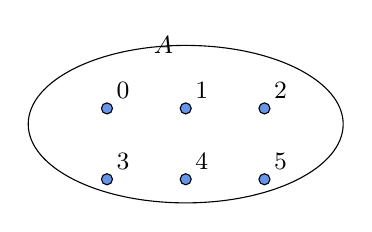
\begin{tikzpicture}[x=2cm,font=\small]
\draw (0,0)circle (1) (0,1) node[ left=1] {$A$};
\begin{scope}[fill=CornflowerBlue, draw=black]
\foreach \x/\xtext in {-.5/0,0/1,.5/2}
\filldraw (\x,.2) circle (2pt) node[above right] {\xtext};
\foreach \y/\ytext in {-.5/3,0/4,.5/5}{
\filldraw (\y,-.7) circle (2pt) node[above right] {\ytext};
}
\end{scope}
\end{tikzpicture}

 \end{center}

 \end{esempio}

 \begin{esempio}
 $B$ è l'insieme delle lettere della parola ``TARTARUGA'', 
 $B=\{t, a, r, u, g\}$.
 \begin{center}
  % (c) 2012 Dimitrios Vrettos - d.vrettos@gmail.com
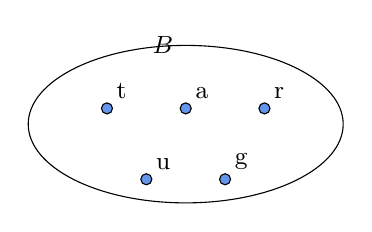
\begin{tikzpicture}[x=2cm,font=\small]
\draw (0,0)circle (1) (0,1) node[ left=1] {$B$};
\begin{scope}[fill=CornflowerBlue, draw=black]
\foreach \x/\xtext in {-.5/t,0/a,.5/r}
\filldraw (\x,.2) circle (2pt) node[above right] {\xtext};
\foreach \y/\ytext in {-.25/u,.25/g}{
\filldraw (\y,-.7) circle (2pt) node[above right] {\ytext};
}
\end{scope}
\end{tikzpicture}

 \end{center}

 \end{esempio}

\end{exrig}

Un insieme può essere rappresentato con una qualsiasi delle
rappresentazioni indicate. Se un insieme è infinito o è costituito
da un numero elevato di elementi la rappresentazione più pratica è
quella per caratteristica.

\begin{exrig}
 \begin{esempio}
 Rappresentare l'insieme~$C$ dei multipli di~5.

 Per caratteristica:~$C=\{n\in\insN/n\text{ è multiplo di }5\}$ oppure
$C=\{n\in\insN/n=5\cdot m,m\in\insN\}$

Tabulare:~$C=\{0, 5, 10, 15, 20, 25, 30, 35,\dots\}$. I puntini di sospensione 
indicano che l'elenco continua.

Rappresentazione con diagramma di Eulero-Venn:
\begin{center}
 % (c) 2012 Dimitrios Vrettos - d.vrettos@gmail.com
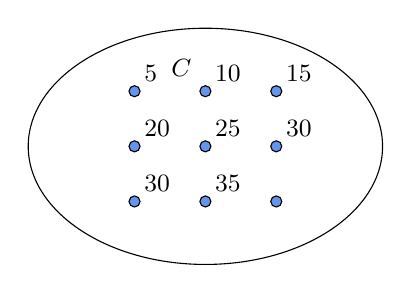
\begin{tikzpicture}[x=1.5cm,font=\small]
    \draw (0,0)circle (1.5) (0,1) node[ left=1.5] {$C$};
    \begin{scope}[fill=CornflowerBlue, draw=black]
\foreach \x/\xtext in {-.6/5,0/10,.6/15}
\filldraw (\x,.7) circle (2pt) node[above right] {\xtext};
\foreach \y/\ytext in {-.6/20,0/25,.6/30}
\filldraw (\y,0) circle (2pt) node[above right] {\ytext};
\foreach \z/\ztext in {-.6/30,0/35,.6/{}}
\filldraw(\z,-.7) circle (2pt) node [above right]  {\ztext};
\end{scope}
\end{tikzpicture}

\end{center}
 \end{esempio}
\end{exrig}

% \ovalbox{\risolvii \ref{ese:6.21}, \ref{ese:6.22}}

% --------------------- Operazioni ---------------------

\section{Operazioni con gli insiemi}
\label{sec:insiemi_operazioni}

\subsection{Sottoinsieme}
\label{subsec:op_sottoinsieme}

Consideriamo l'insieme~$A$ degli abitanti di Milano e l'insieme~$B$ degli 
abitanti di Milano con età superiore ai~40 anni. Gli abitanti ultra 
quarantenni di Milano fanno parte della popolazione di Milano, cioè tutti gli
elementi dell'insieme~$B$ sono anche elementi di~$A$: si dice che~$B$ è 
sottoinsieme di~$A$, si scrive~$B\subseteq A$.

Nel caso in cui tutti gli elementi di~$Y$ siano elementi di~$X$ e tutti gli 
elementi di~$X$ siano elementi di
$Y$ si ha che~$X=Y$, e~$Y$ si dice \emph{sottoinsieme improprio} di~$X$.
Se~$X\subseteq Y$ e~$Y\subseteq X$, allora~$Y=X$.

Tra i sottoinsiemi di un insieme si considera anche
l'insieme vuoto~$\emptyset $, cioè qualunque sia l'insieme~$X$ risulta 
che~$\emptyset \subset X$.
L'insieme vuoto è considerato un \emph{sottoinsieme improprio} di qualunque 
insieme.
Ogni insieme è sottoinsieme improprio di se stesso.

Se~$Y$ è un sottoinsieme di~$X$ e~$X$ ha altri elementi oltre a quelli di~$Y$
si dice che~$Y$ è un \emph{sottoinsieme proprio} di~$X$ e si scrive~$Y\subset X$.
La scrittura~$A\subseteq B$ si usa quando non si sa in modo certo se~$A=B$ o
$A\subset B$.

\begin{definizione}
Dati due insiemi~$X$ e~$Y$, si dice che~$Y$ è un \emph{sottoinsieme} di~$X$
se ogni elemento di~$Y$ è anche elemento di~$X$.

In simboli:~$Y\subseteq X$, che si legge
``$Y$ è incluso in~$X$'' o ``$Y$ è sottoinsieme di~$X$''.
\end{definizione}

La rappresentazione con un diagramma di Eulero-Venn è la seguente:
\begin{center}
% (c) 2012 Dimitrios Vrettos - d.vrettos@gmail.com
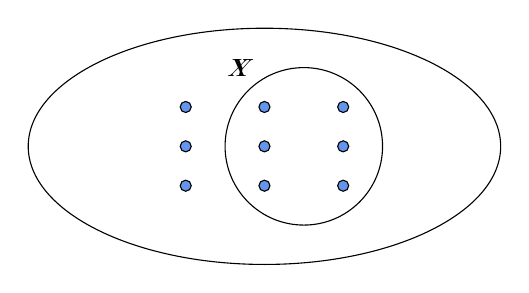
\begin{tikzpicture}[x=2cm,font=\small, fill=CornflowerBlue]
    \draw (0,0)circle (1.5) (0,1) node[ left=1.5] {$X$};
\foreach \x in {-.5,0,.5}
\foreach \y in {-.5,0,.5}
\filldraw (\x,\y) circle (2pt) node[above right] {};
\begin{scope}[y=2cm]]
    \draw (0.25,0)circle (.5) (0,.5) node[left=.1] {$Y$};
\end{scope}
\end{tikzpicture}

\end{center}
Se~$a$ è un elemento del sottoinsieme~$Y$, allora lo sarà anche 
dell'insieme~$X$:
\begin{center}
se~$a\in Y$ e~$Y\subseteq X$, allora~$a\in X$.
\end{center}

Dalla stessa definizione, si deduce che ogni insieme è sottoinsieme di
se stesso, in simboli~$X\subseteq X$.
Tra i sottoinsiemi di un insieme si considera anche
l'insieme vuoto. Cioè, qualunque sia
l'insieme~$X$ risulta~$\emptyset \subseteq X$.

\begin{exrig}

\begin{esempio}
Consideriamo l'insieme~$X=\{\text{lettere della parola ``autunno''}\}$ e
l'insieme~$Y=\{\text{lettere della parola ``notaio''}\}$ possiamo affermare 
che ``ogni''
elemento di~$Y$ è anche elemento di~$X$? La risposta è negativa:~$i\in Y$ ma
$i\notin X$ quindi~$Y$ non è sottoinsieme di~$X$ e si scrive~$Y\not\subset X$.
\end{esempio}

\begin{esempio}
Sia~$A$ l'insieme delle lettere dell'alfabeto italiano e~$V$
l'insieme delle vocali, allora si può scrivere
$V\subset A$ cioè~$V$ è un sottoinsieme proprio di~$A$,
come si può anche vedere dalla rappresentazione grafica.
\begin{center}
 % (c) 2012 Dimitrios Vrettos - d.vrettos@gmail.com
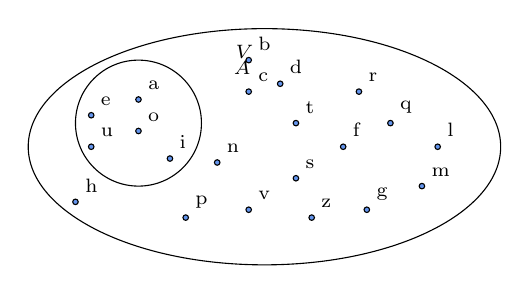
\begin{tikzpicture}[x=2cm,font=\scriptsize, fill=CornflowerBlue]
    \draw (0,0)circle (1.5) (0,1) node[ left=1.5] {$A$};
\filldraw (-.8,.6) circle (1pt) node[above right] {a};
\filldraw (-1.1,.4) circle (1pt) node[above right] {e};
\filldraw (-.6,-.15) circle (1pt) node[above right] {i};
\filldraw (-.8,.2) circle (1pt) node[above right] {o};
\filldraw (-1.1,0) circle (1pt) node[above right] {u};

\filldraw (-.1,1.1) circle (1pt) node[above right] {b};
\filldraw (-.1,.7) circle (1pt) node[above right] {c};
\filldraw (.1,.8) circle (1pt) node[above right] {d};
\filldraw (.5,0) circle (1pt) node[above right] {f};
\filldraw (.65,-.8) circle (1pt) node[above right] {g};
\filldraw (-1.2,-.7) circle (1pt) node[above right] {h};
\filldraw (1.1,0) circle (1pt) node[above right] {l};
\filldraw (1,-.5) circle (1pt) node[above right] {m};
\filldraw (-.3,-.2) circle (1pt) node[above right] {n};
\filldraw (-.5,-.9) circle (1pt) node[above right] {p};
\filldraw (.8,.3) circle (1pt) node[above right] {q};
\filldraw (.6,.7) circle (1pt) node[above right] {r};
\filldraw (.2,-.4) circle (1pt) node[above right] {s};
\filldraw (.2,.3) circle (1pt) node[above right] {t};
\filldraw (-.1,-.8) circle (1pt) node[above right] {v};
\filldraw (.3,-.9) circle (1pt) node[above right] {z};
 \begin{scope}[y=2cm]]
     \draw (-.8,.15)circle (.4) (0,.6) node[left=.4] {$V$};
 \end{scope}
\end{tikzpicture}

\end{center}

\end{esempio}

\begin{esempio}
Sia~$C=\{1\}$, allora~$C$ non ha sottoinsiemi propri;
mentre i suoi sottoinsiemi impropri sono~$C=\{1\}$ e
l'insieme vuoto~$\emptyset $.
\end{esempio}

\begin{esempio}
Sia~$A$ l'insieme delle auto esposte in un
autosalone e~$U$ l'insieme delle auto usate
esposte nello stesso autosalone. Si ha che~$U$ è un
sottoinsieme di~$A$, ma senza avere ulteriori informazioni non
possiamo escludere che tutte le auto esposte siano usate, dobbiamo
perciò scrivere~$U\subseteq A$. Se invece sappiamo che nessuna
auto esposta è usata, allora~$U=\emptyset $.
\end{esempio}
\end{exrig}

% \ovalbox{\risolvi \ref{ese:7.1}}

\subsection{Insieme delle parti}
\label{subsec:op_parti}

Consideriamo l'insieme~$A$ dei numeri naturali
compresi tra~0 e~100, a partire da questo insieme possiamo formare
gruppi costituiti dai soli numeri multipli di~10, dai numeri pari, da
quelli dispari, da quelli divisibili per~7 e così via. Quindi con gli
elementi dell'insieme~$A$ possiamo formare molti
altri insiemi che sono sottoinsiemi di~$A$.

\begin{exrig}
 \begin{esempio}
Determinare tutti i sottoinsiemi di~$A=\{1,2,3\}$.

$\emptyset \subset A$, infatti l'insieme vuoto è un
sottoinsieme di qualunque insieme.

Elenchiamo tutti i sottoinsiemi costituiti da un solo 
elemento:~\{1\},~\{2\},~\{3\}.
Elenchiamo ora tutti i sottoinsiemi costituiti da due 
elementi:~\{1,2\},~\{1,3\},~\{2,3\}.
L'unico sottoinsieme costituito da tre elementi è~$A$ stesso, possiamo 
scrivere:~$\{1,2,3\}\subseteq A$. In tutto 8 sottoinsiemi.
 \end{esempio}

\end{exrig}

\begin{definizione}
Dato un insieme~$A$, si chiama \emph{insieme delle parti} l'insieme che ha 
come elementi tutti i sottoinsiemi propri ed impropri di~$A$. In simboli:
$\wp (A)$.
\end{definizione}

L'insieme delle parti di un insieme A ha sempre come
elementi~$\emptyset $ e~$A$ quindi~$\emptyset\in\wp (A)$ e
$A\in\wp (A)$.

Il numero degli elementi di~$\wp (A)$, cioè dei suoi possibili
sottoinsiemi, propri e impropri, dipende dal numero degli elementi di~$A$.

\begin{exrig}
 \begin{esempio}
 L'insieme vuoto ha come unico sottoinsieme se stesso,
quindi~$\wp (\emptyset )=\{\emptyset \}$.
 \end{esempio}

\begin{esempio}
 Dato l'insieme~$A=\{a\}$, i suoi possibili sottoinsiemi
propri ed impropri sono:~$S_{1}=\emptyset$, $S_{2}=\{a\}$
allora~$\wp (A)=\{S_{1},S_{2}\}$.
 \end{esempio}

\begin{esempio}
 Dato l'insieme~$B=\{\text{matita, penna}\}$ i
suoi possibili sottoinsiemi propri ed impropri sono:~$S_{1}=\emptyset$,
$S_{2}=B=\{\text{matita, penna}\}$, $S_{3}=\{\text{matita}\}$,
$S_{4}=\{\text{penna}\}$
allora~$\wp (A)=\{S_{1}, S_{2}, S_{3}, S_{4}\}$.
 \end{esempio}

\begin{esempio}
 Dato l'insieme~$B=\{1,2,3\}$, i suoi possibili
sottoinsiemi propri ed impropri sono:~$S_{1}=\emptyset$,
$S_{2}=B=\{1,2,3\}$, $S_{3}=\{1\}$, $S_{4}=\{2\}$, $S_{5}=\{3\}$,
$S_{6}=\{1,2\}$, $S_{7}=\{1,3\}$, $S_{8}=\{2,3\}$
allora~$\wp (A)=\{S_{1}, S_{2}, S_{3}, S_{4}, S_{5}, S_{6}, S_{7,}, S_{8}\}$.
 \end{esempio}
 \end{exrig}

 Riassumendo:
\begin{itemize*}
\item se~$A=\emptyset $ l'insieme delle parti ha~1 solo elemento;
\item se~$A$ ha~1 elemento allora l'insieme delle parti ha~2 elementi;
\item se~$A$ ha~2 elementi, l'insieme delle parti ne ha~4;
\item se~$A$ ha~3 elementi, l'insieme delle parti ne ha~8.
\end{itemize*}

Generalizzando, se~$A$ ha~$n$ elementi, l'insieme delle parti ne ha~$2^{n}$.

% \vspazio\ovalbox{\risolvii \ref{ese:7.2}, \ref{ese:7.3}, \ref{ese:7.4}, \ref{ese:7.5}, \ref{ese:7.6}}

\subsection{Insieme unione}
\label{subsec:op_unione}

Prendiamo l'insieme~$\insP$ dei numeri pari e l'insieme~$\insD$ dei numeri 
dispari; allora l'insieme~$\insN$ dei numeri naturali è dato dall'unione dei 
due insiemi~$\insP$ e~$\insD$.

\begin{definizione}
Dati due insiemi~$A$ e~$B$, si dice
\emph{insieme unione} l'insieme~$C$, composto da tutti gli elementi 
appartenenti ad $A$ o a~$B$ o a entrambi.
In simboli:~$C=A\cup B$, si legge ``$A$ unito a~$B$''
o ``$A$ unione~$B$''.
\end{definizione}
\begin{center}
 % (c) 2012 Dimitrios Vrettos - d.vrettos@gmail.com
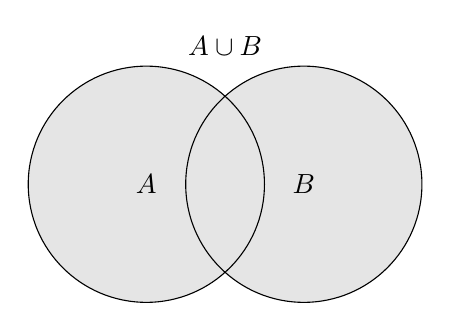
\begin{tikzpicture}[filled/.style={fill=circle area, draw=black, thin}]

\def\firstcircle{(0,0) circle (1.5cm)}
\def\secondcircle{(0:2cm) circle (1.5cm)}

\definecolor{circle area}{gray}{.9}

 \draw[filled] \firstcircle node {$A$}
                  \secondcircle node {$B$};
 \node[anchor=south] at (current bounding box.north) {$A \cup B$};
\end{tikzpicture}

\end{center}


Mediante la proprietà caratteristica si 
scrive:~$C=A\cup B=\{x/(x\in A)\text{ o }(x\in B)\}$.

\subsubsection{Proprietà dell'unione tra insiemi}

\begin{enumeratea}
\item $A\cup B=B\cup A$: proprietà \emph{commutativa} dell'unione;
\item $(A\cup B)\cup C=A\cup (B\cup C)$: proprietà \emph{associativa} 
dell'unione;
\item se~$B\subset A$, allora~$A\cup B=A$
\item $A\cup \emptyset =A$
\item $A\cup A=A$: proprietà di \emph{idempotenza} dell'unione.
\end{enumeratea}

\begin{exrig}
 \begin{esempio}
Siano~$D=\{1,3,5\}$ e~$P=\{2,4,6\}$ allora~$N=P\cup D=\{1,2,3,4,5,6\}$.
\begin{center}
 % (c) 2012 Dimitrios Vrettos - d.vrettos@gmail.com
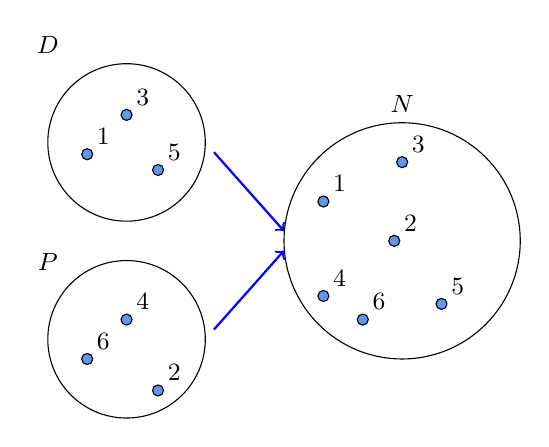
\begin{tikzpicture}[font=\small, fill=CornflowerBlue]
\draw (0,1.25)circle (1) (-1,2.25) node[above] {$D$};
\draw(0,-1.25) circle (1) (-1,-.5) node [above]  {$P$};
\draw (3.5,0) circle (1.5) (3.5,1.5) node [above]  {$N$};

\filldraw (-.5,1.1) circle (2pt) node[above right] {1};
\filldraw (0,1.6) circle (2pt) node[above right] {3};
\filldraw (.4,.9) circle (2pt) node[above right] {5};

\filldraw (-.5,-1.5) circle (2pt) node[above right] {6};
\filldraw (0,-1) circle (2pt) node[above right] {4};
\filldraw (.4,-1.9) circle (2pt) node[above right] {2};

\filldraw (2.5,.5) circle (2pt) node[above right] {1};
\filldraw (3.5,1) circle (2pt) node[above right] {3};
\filldraw (4,-.8) circle (2pt) node[above right] {5};

\filldraw (3,-1) circle (2pt) node[above right] {6};
\filldraw (2.5,-.7) circle (2pt) node[above right] {4};
\filldraw (3.4,0) circle (2pt) node[above right] {2};

\node (d) at (1,1.25) {};
\node (p) at (1,-1.25) {};
\node (n) at (2,0) {};

\begin{scope}[blue, ->,thick]
\draw (d)--(n.north);
\draw (p)--(n.south);
\end{scope}
\end{tikzpicture}

\end{center}

\end{esempio}

\begin{esempio}
Siano~$X=\{\text{do, re, mi, fa, sol, la, si}\}$
e~$Y=\{\text{do, re, mi}\}$, allora, 
poiché $Y\subset X$, $W=X\cup Y=X=\{\text{do, re, mi, fa, sol, la, si}\}$.
\begin{center}
 % (c) 2012 Dimitrios Vrettos - d.vrettos@gmail.com
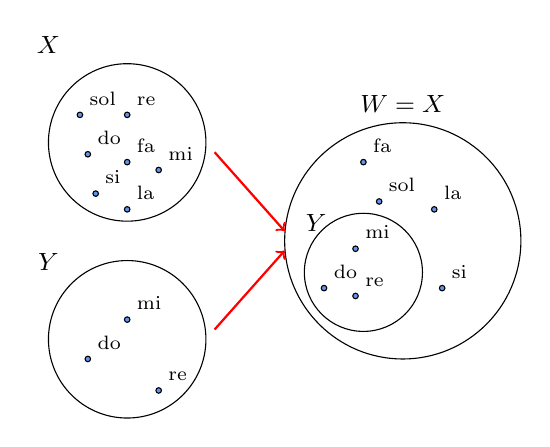
\begin{tikzpicture}[fill=CornflowerBlue]
\begin{scope}[font=\small]
\draw (0,1.25)circle (1) (-1,2.25) node[above] {$X$};
\draw(0,-1.25) circle (1) (-1,-.5) node [above]  {$Y$};
\draw (3.5,0) circle (1.5) (3.5,1.5) node [above]  {$W=X$};
\draw(3,-.4) circle (.75) (2.4,0) node [above] {$Y$};
\end{scope}
\begin{scope}[font=\scriptsize]
\filldraw (-.5,1.1) circle (1pt) node[above right] {do};
\filldraw (0,1.6) circle (1pt) node[above right] {re};
\filldraw (.4,.9) circle (1pt) node[above right] {mi};
\filldraw (0,1) circle (1pt) node[above right] {fa};
\filldraw (-.6,1.6) circle (1pt) node[above right] {sol};
\filldraw (0,.4) circle (1pt) node[above right] {la};
\filldraw (-.4,.6) circle (1pt) node[above right] {si};

\filldraw (-.5,-1.5) circle (1pt) node[above right] {do};
\filldraw (0,-1) circle (1pt) node[above right] {mi};
\filldraw (.4,-1.9) circle (1pt) node[above right] {re};

\filldraw (2.5,-.6) circle (1pt) node[above right] {do};
\filldraw (2.9,-.7) circle (1pt) node[above right] {re};
\filldraw (2.9,-.1) circle (1pt) node[above right] {mi};
\filldraw (3,1) circle (1pt) node[above right] {fa};
\filldraw (3.2,.5) circle (1pt) node[above right] {sol};
\filldraw (3.9,.4) circle (1pt) node[above right] {la};
\filldraw (4,-.6) circle (1pt) node[above right] {si};
\end{scope}
\node (x) at (1,1.25) {};
\node (y) at (1,-1.25) {};
\node (w) at (2,0) {};

\begin{scope}[red, ->,thick]
\draw (x)--(w.north);
\draw (y)--(w.south);
\end{scope}
\end{tikzpicture}

\end{center}

\end{esempio}
\end{exrig}

% \ovalbox{\risolvii \ref{ese:7.7}, \ref{ese:7.8}, \ref{ese:7.9}}

\subsection{Insieme intersezione}
\label{subsec:op_intersezione}

\begin{exrig}
\vspace{1.05ex}
 \begin{esempio}
Se~$A$ è l'insieme delle lettere della parola ``matematica'' e~$B$ è 
l'insieme delle lettere della parola ``materia''. 
Quali elementi di~$A$ stanno in~$B$? Quali elementi di~$B$ stanno in~$A$? 
Quali sono gli elementi che stanno in entrambi gli insiemi?

\begin{itemize*}
 \item L'insieme degli elementi di~$A$ che stanno in~$B$ è~\{m, a, t, e, i\};
 \item l'insieme degli elementi di~$B$ che stanno in~$A$ è~\{m, a, t, e, i\};
 \item l'insieme degli elementi che stanno sia in~$A$ sia in~$B$ 
 è~\{m, a, t, e, i\}.
\end{itemize*}
\end{esempio}
\end{exrig}

\begin{definizione}
Dati due insiemi~$A$ e~$B$, si dice \emph{insieme intersezione} di~$A$ e~$B$, 
l'insieme~$C$ composto da tutti gli elementi appartenenti contemporaneamente 
ad~$A$ e a~$B$, ossia comuni a entrambi.
In simboli:~$C=A\cap B$, che si legge ``$A$ intersecato a~$B$'' o ``$A$ 
intersezione~$B$''.
\end{definizione}
\begin{center}
 % (c) 2012 Dimitrios Vrettos - d.vrettos@gmail.com
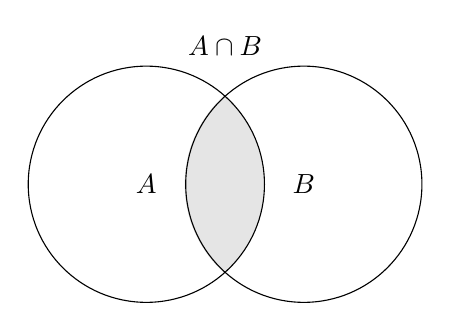
\begin{tikzpicture}[filled/.style={fill=circle area, draw=circle edge, thick}]
\def\firstcircle{(0,0) circle (1.5cm)}
\def\secondcircle{(0:2cm) circle (1.5cm)}

\definecolor{circle edge}{gray}{0.9}
\definecolor{circle area}{gray}{0.9}
    \begin{scope}
        \clip \firstcircle;
        \fill[filled] \secondcircle;
    \end{scope}
    \draw\firstcircle node {$A$};
    \draw \secondcircle node {$B$};
    \node[anchor=south] at (current bounding box.north) {$A \cap B$};
\end{tikzpicture}

\end{center}
Mediante proprietà caratteristica si 
scrive:~$C=A\cap B=\{x/(x\in A)\text{ e }(x\in B)\}$.

Se~$A\cap B=\emptyset $, ossia se~$A$ e~$B$ non hanno
elementi in comune, i due insiemi si dicono \emph{disgiunti}.

\subsubsection{Proprietà dell'intersezione tra insiemi}

\begin{enumeratea}
\item $A\cap B=B\cap A$: proprietà \emph{commutativa} dell'intersezione;
\item $(A\cap B)\cap C=A\cap (B\cap C)$: proprietà \emph{associativa} 
dell'intersezione;
\item Se~$B\subset A$, allora~$A\cap B=B$
\item $A\cap \emptyset =\emptyset$
\item $A\cap A=A$: proprietà di \emph{idempotenza} dell'intersezione;
\item $\emptyset \cap \emptyset =\emptyset$.
\end{enumeratea}

\subsection[Proprietà distributiva]
{Proprietà distributiva tra intersezione e unione}

\begin{enumeratea}
\item $A\cap (B\cup C)=(A\cap B)\cup (A\cap C)$: 
proprietà \emph{distributiva} dell'intersezione rispetto l'unione;
\item $A\cup (B\cap C)=(A\cup B)\cap (A\cup C)$: 
proprietà \emph{distributiva} dell'unione rispetto l'intersezione.
\end{enumeratea}

\begin{exrig}
 \begin{esempio}
Siano~$X=\{\text{do, re, mi. fa, sol, la, si}\}$
e~$Y=\{\text{do, re, mi}\}$. Allora poiché, 
$Y\subset X$, si ha:~$W=X\cap Y=Y=\{\text{do, re, mi}\}$.
 \end{esempio}

 \begin{esempio}
Siano~$D=\{1,3,5\}$ e~$P=\{2,4,6\}$ allora~$N=P\cap D=\emptyset$.
\begin{center}
 % (c) 2012 Dimitrios Vrettos - d.vrettos@gmail.com
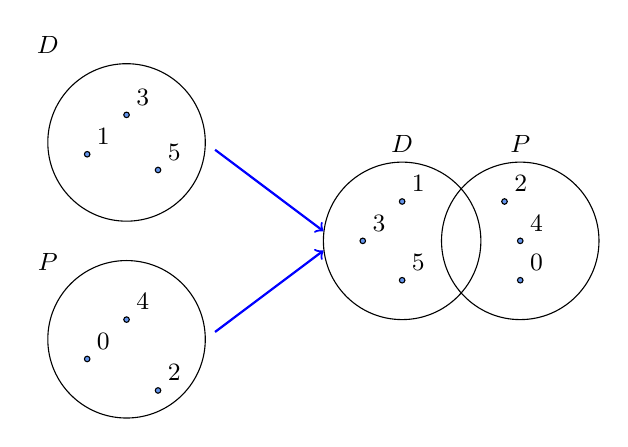
\begin{tikzpicture}[font=\small, fill=CornflowerBlue]
\draw (0,1.25)circle (1) (-1,2.25) node[above] {$D$};
\draw(0,-1.25) circle (1) (-1,-.5) node [above]  {$P$};
\draw (3.5,0) circle (1) (3.5,1) node [above]  {$D$};
\draw (5,0) circle (1) (5,1) node [above]  {$P$};

\filldraw (-.5,1.1) circle (1pt) node[above right] {1};
\filldraw (0,1.6) circle (1pt) node[above right] {3};
\filldraw (.4,.9) circle (1pt) node[above right] {5};

\filldraw (-.5,-1.5) circle (1pt) node[above right] {0};
\filldraw (0,-1) circle (1pt) node[above right] {4};
\filldraw (.4,-1.9) circle (1pt) node[above right] {2};

\filldraw (3.5,.5) circle (1pt) node[above right] {1};
\filldraw (3,0) circle (1pt) node[above right] {3};
\filldraw (3.5,-.5) circle (1pt) node[above right] {5};

\filldraw (5,-.5) circle (1pt) node[above right] {0};
\filldraw (5,0) circle (1pt) node[above right] {4};
\filldraw (4.8,.5) circle (1pt) node[above right] {2};

\node (d) at (1,1.25) {};
\node (p) at (1,-1.25) {};
\node (n) at (2.5,0) {};

\begin{scope}[blue, ->,thick]
\draw (d)--(n.north);
\draw (p)--(n.south);
\end{scope}
\end{tikzpicture}

\end{center}
 \end{esempio}
\end{exrig}

% \ovalbox{\risolvii \ref{ese:7.10}, \ref{ese:7.11}, \ref{ese:7.12}, 
% \ref{ese:7.13}}

\subsection{Insieme differenza}
\label{subsec:op_differenza}

Consideriamo gli insiemi~$A$ e~$B$ formati rispettivamente
dalle lettere dell'alfabeto italiano e dalle
consonanti dell'alfabeto italiano cioè:
$A=$\{a, b, c, d, e, f, g, h, i, l, m, n, o, p, q, r, s, t, u, v, z\} e
$B=$\{b, c, d, f, g, h, l, m, n, p, q, r, s, t, v, z\}, le lettere 
``a, e, i, o, u'' che compaiono nell'insieme~$A$ ma non in~$B$ formano un 
nuovo insieme chiamato insieme \emph{differenza}.

\begin{definizione}
 Dati due insiemi~$A$ e~$B$, si dice \emph{insieme differenza} l'insieme~$C$, 
 composto da tutti gli elementi di~$A$ che non appartengono a~$B$. 
 In simboli:~$C=A-B$ che si legge ``$A$ differenza~$B$''.
\end{definizione}

\begin{center}
% (c) 2012 Dimitrios Vrettos - d.vrettos@gmail.com
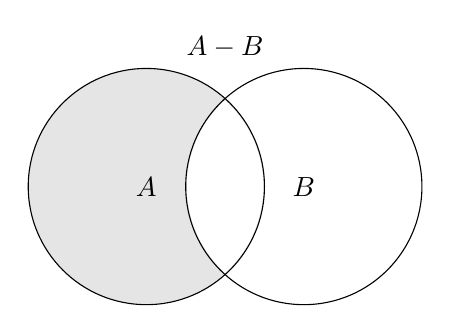
\begin{tikzpicture}[filled/.style={fill=circle area, draw=circle edge, thick}]
\def\firstcircle{(0,0) circle (1.5cm)}
\def\secondcircle{(0:2cm) circle (1.5cm)}

\definecolor{circle edge}{gray}{0.9}
\definecolor{circle area}{gray}{0.9}
\begin{scope}
\clip \firstcircle;
\draw[filled, even odd rule] \firstcircle node {$A$}
\secondcircle;
\end{scope}
\draw\firstcircle;
\draw \secondcircle node {$B$};
\node[anchor=south] at (current bounding box.north) {$A- B$};
\end{tikzpicture}

\end{center}
Mediante proprietà caratteristica si 
scrive:~$C=A-B=\{x/(x\in A)\text{ e }(x\notin B)\}$.

\subsubsection{Proprietà della differenza tra insiemi}

\begin{enumeratea}
\item Se~$A\cap B=\emptyset $, ossia sono disgiunti allora~$A-B=A$, e~$B-A=B$
\item se~$B\subset A$, ossia~$B$ è sottoinsieme proprio 
 di~$A$ allora~$B-A=\emptyset $
\item $A-A=\emptyset$
\item $A-\emptyset =A$.
\end{enumeratea}

\begin{exrig}
 \begin{esempio}
Siano~$A=\{8, 9, 10, 12, 13\}$ e~$B=\{9, 10, 11, 13\}$ allora
$C=A-B=\{8, 12\}$ e~$D=B-A=\{11\}$.
 \end{esempio}
\end{exrig}

Poiché $A-B\neq B-A$ nella differenza non vale la proprietà
commutativa.

\begin{exrig}
 \begin{esempio}
Siano~$D=\{1, 3, 5\}$ e~$P=\{0, 2, 4\}$. I due insiemi sono 
disgiunti~$P\cap D=\emptyset$ allora~$D-P=\{1,3,5\}=D$ e~$P-D=\{0,2,4\}=P$.
\begin{center}
 % (c) 2012 Dimitrios Vrettos - d.vrettos@gmail.com
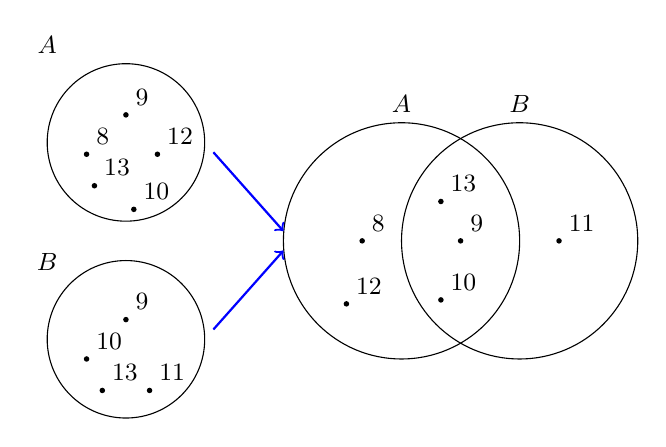
\begin{tikzpicture}[font=\small]
\draw (0,1.25)circle (1) (-1,2.25) node[above] {$A$};
\draw(0,-1.25) circle (1) (-1,-.5) node [above]  {$B$};
\draw (3.5,0) circle (1.5) (3.5,1.5) node [above]  {$A$};
\draw (5,0) circle (1.5) (5,1.5) node [above]  {$B$};

\fill (-.5,1.1) circle (1pt) node[above right] {8};
\fill (0,1.6) circle (1pt) node[above right] {9};
\fill (.4,1.1) circle (1pt) node[above right] {12};
\fill (-.4,.7) circle (1pt) node[above right] {13};
\fill (.1,.4) circle (1pt) node[above right] {10};

\fill (-.5,-1.5) circle (1pt) node[above right] {10};
\fill (0,-1) circle (1pt) node[above right] {9};
\fill (.3,-1.9) circle (1pt) node[above right] {11};
\fill (-.3,-1.9) circle (1pt) node[above right] {13};

\fill (4,.5) circle (1pt) node[above right] {13};
\fill (3,0) circle (1pt) node[above right] {8};
\fill (2.8,-.8) circle (1pt) node[above right] {12};

\fill (4,-.75) circle (1pt) node[above right] {10};
\fill (4.25,0) circle (1pt) node[above right] {9};
\fill (5.5,0) circle (1pt) node[above right] {11};

\node (a) at (1,1.25) {};
\node (b) at (1,-1.25) {};
\node (n) at (2,0) {};

\begin{scope}[blue, ->,thick]
\draw (a)--(n.north);
\draw (b)--(n.south);
\end{scope}
\end{tikzpicture}

\end{center}
 \end{esempio}

 \begin{esempio}
Siano~$X=\{\text{do, re, mi, fa, sol, la, si}\}$
e~$Y=\{\text{do, re, mi}\}$ allora poiché
$Y\subset X$, $W=X-Y=\{\text{fa, sol, la, si}\}$.
\begin{center}
 % (c) 2012 Dimitrios Vrettos - d.vrettos@gmail.com
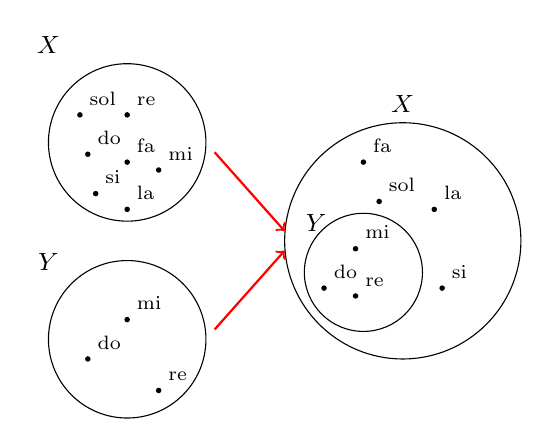
\begin{tikzpicture}
\begin{scope}[font=\small]
\draw (0,1.25)circle (1) (-1,2.25) node[above] {$X$};
\draw(0,-1.25) circle (1) (-1,-.5) node [above]  {$Y$};
\draw (3.5,0) circle (1.5) (3.5,1.5) node [above]  {$X$};
\draw(3,-.4) circle (.75) (2.4,0) node [above] {$Y$};
\end{scope}
\begin{scope}[font=\scriptsize]
\fill (-.5,1.1) circle (1pt) node[above right] {do};
\fill (0,1.6) circle (1pt) node[above right] {re};
\fill (.4,.9) circle (1pt) node[above right] {mi};
\fill (0,1) circle (1pt) node[above right] {fa};
\fill (-.6,1.6) circle (1pt) node[above right] {sol};
\fill (0,.4) circle (1pt) node[above right] {la};
\fill (-.4,.6) circle (1pt) node[above right] {si};

\fill (-.5,-1.5) circle (1pt) node[above right] {do};
\fill (0,-1) circle (1pt) node[above right] {mi};
\fill (.4,-1.9) circle (1pt) node[above right] {re};

\fill (2.5,-.6) circle (1pt) node[above right] {do};
\fill (2.9,-.7) circle (1pt) node[above right] {re};
\fill (2.9,-.1) circle (1pt) node[above right] {mi};
\fill (3,1) circle (1pt) node[above right] {fa};
\fill (3.2,.5) circle (1pt) node[above right] {sol};
\fill (3.9,.4) circle (1pt) node[above right] {la};
\fill (4,-.6) circle (1pt) node[above right] {si};
\end{scope}
\node (x) at (1,1.25) {};
\node (y) at (1,-1.25) {};
\node (w) at (2,0) {};

\begin{scope}[red, ->,thick]
\draw (x)--(w.north);
\draw (y)--(w.south);
\end{scope}
\end{tikzpicture}

\end{center}
 \end{esempio}
\end{exrig}

% \ovalbox{\risolvi \ref{ese:7.14}}

\subsection{Insieme complementare}
\label{subsec:op_complementare}

Sia~$W=\{\text{sabato, domenica}\}$ l'insieme dei giorni della settimana che 
non finiscono per ``dì''.
L'insieme~$W$ può essere considerato come sottoinsieme dell'insieme~$G$ 
formato da tutti i giorni della settimana
$G=$\{lunedì, martedì, mercoledì, giovedì, venerdì, sabato, domenica\}.
L'insieme degli elementi di~$G$ che non appartengono a~$W$ forma
un insieme che chiameremo {\emph{complementare} di~$W$ rispetto a~$G$. 
L'insieme~$G$ invece si dice in questo caso insieme \emph{universo}. 
Ad esempio nella rappresentazione caratteristica~$A=\{x\in N/x\le~100\}$,
$N$ è l'insieme universo di~$A$.

\begin{definizione}
Dato un insieme~$A$, uno dei possibili insiemi che
contengono~$A$ come sottoinsieme si dice
\emph{insieme universo} o \emph{insieme ambiente}.
\end{definizione}

\begin{definizione}
Dato l'insieme~$A$ e scelto~$U$ come suo insieme universo, l'insieme degli 
elementi di $U$ che non appartengono ad~$A$ si dice 
\emph{insieme complementare} di~$A$ rispetto a~$U$. 
In simboli:~$\overline{A}$ oppure~$\overline{A}_{U}$ oppure~$\complement_{U}A$.
\end{definizione}

\begin{multicols}{2}
Il diagramma di Eulero-Venn dell'insieme complementare è:
\begin{center}
% (c) 2012 Dimitrios Vrettos - d.vrettos@gmail.com
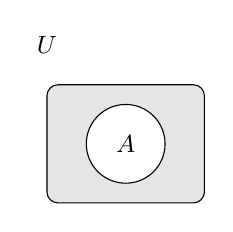
\begin{tikzpicture}[x=5mm,y=5mm,font=\small]
\definecolor{circle area}{gray}{0.9}
\draw[rounded corners, fill=circle area] (0,0) rectangle (4,3) (0,4) node {$U$};
\draw[fill=white](2,1.5) circle (1) (2,1.5) node {$A$};
\end{tikzpicture}

\end{center}
Nella figura la parte in grigio è il complementare di~$A$ rispetto a~$U$, 
cioè~${\overline{A}}_{U}$.
Come si può vedere dal disegno, essendo~$A\subseteq U$ il complementare 
coincide con la differenza tra insiemi: ${\overline{A}}_{U}=U-A$.
\end{multicols}

\begin{exrig}
 \begin{esempio}
 Insiemi complementari.
\begin{enumeratea}
\item Il complementare dell'insieme~$D$ dei numeri dispari rispetto 
all'insieme~$\insN$ dei numeri naturali è
l'insieme~$P$ dei numeri pari:~${\overline{D}}_{\insN}=P$
\item Il complementare dell'insieme~$V$ delle vocali dell'alfabeto italiano 
rispetto all'insieme~$A$ delle lettere dell'alfabeto italiano è 
l'insieme~$C$ delle consonanti: ${\overline{V}}_{U}=C$
\item Dati gli insiemi~$U=\{x\in N/1\le x\le~10\}$ 
 e~$B=\{x\in N/1\le x\le~5\}$, poiché $B\subset U$
 si può determinare~${\overline{B}}_{U}=\{x\in N/6\le x\le~10\}$.
\end{enumeratea}
 \end{esempio}
\end{exrig}

% \ovalbox{\risolvii \ref{ese:7.15}, \ref{ese:7.16}, \ref{ese:7.17}}

\subsection{Leggi di De Morgan}
\label{subsec:op_demorgan}

Dati due insiemi~$A$ e~$B$ ci sono alcune proprietà,
dette \emph{leggi di De Morgan} che semplificano lo svolgimento di alcune 
operazioni:


\begin{enumeratea}
\item $\overline{{A\cap B}}=\overline{A}\cup \overline{B}$: 
Prima legge di De Morgan;
\item $\overline{{A\cup B}}=\overline{A}\cap \overline{B}$: 
Seconda legge di De Morgan.
\end{enumeratea}

Dimostriamo la prima legge di De Morgan utilizzando i diagrammi di Eulero-Venn.
\begin{center}
 % (c) 2012 Dimitrios Vrettos - d.vrettos@gmail.com
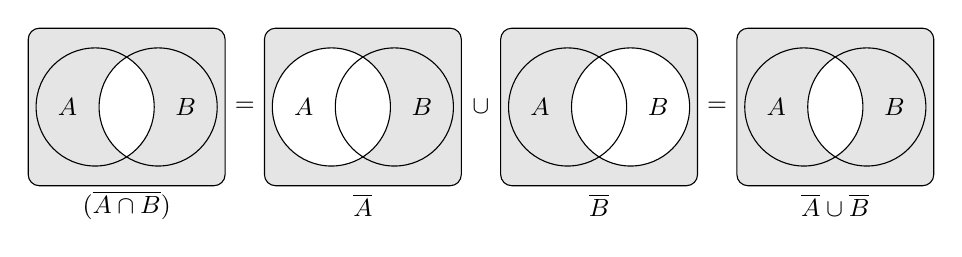
\begin{tikzpicture}[x=5mm,y=5mm,font=\small, outline/.style={draw=circle edge}]
\definecolor{circle area}{gray}{0.9}
\definecolor{circle edge}{rgb}{0,0,0}

\def\firstcircle{(1.7,2) circle (1.5)}
\def\secondcircle{(3.3,2) circle (1.5)}

\begin{scope}[rounded corners]
\foreach \i in {0,6,12,18}
\draw[fill=circle area] (\i,0) rectangle (\i+5,4);
\end{scope}

\begin{scope}]
\begin{scope}
\clip \firstcircle;
\fill[white] \secondcircle;
\end{scope}
\draw[outline] \firstcircle;
\draw[outline] \secondcircle;
\end{scope}

\begin{scope}[xshift=30mm]
\begin{scope}
\clip \firstcircle;
\fill[white] \firstcircle;
\end{scope}
 \draw[outline]  \firstcircle;
\draw[outline] \secondcircle;
\end{scope}

\begin{scope}[xshift=60mm]
\begin{scope}
\clip \secondcircle;
\fill[white] \secondcircle;
\end{scope}
 \draw[outline]  \firstcircle;
\draw[outline] \secondcircle;
\end{scope}

\begin{scope}[xshift=90mm]
\begin{scope}
\clip \firstcircle;
\fill[white] \secondcircle;
\end{scope}
\draw[outline] \firstcircle;
 \draw[outline] \secondcircle;
\end{scope}

\foreach \x/\xtext in {5.5/$=$,11.5/$\cup$,17.5/$=$}
	\node  at (\x,2) {\xtext};

\foreach \y in {1,7,13,19}
\node  at (\y,2) {$A$};

\foreach \z in {4,10,16,22}
\node  at (\z,2) {$B$};

\foreach \j/\jtext in {2.5/(\overline{A\cap B}),8.5/\overline{A},14.5/\overline{B},20.5/\overline{A}\cup\overline{B}
}
\node  at (\j,-.5) {$\jtext$};
\end{tikzpicture}

\end{center}

% \ovalbox{\risolvi \ref{ese:7.18}}

\subsection{Prodotto cartesiano fra insiemi}
\label{subsec:op_cartesiano}

Supponiamo che la partita di calcio Lecce~-~Juventus sia terminata~3-2; 
in questo caso il risultato della partita non rappresenta un insieme di 
numeri dato che nella rappresentazione di un insieme 
scrivere~$\{3,2\}$ e~$\{2,3\}$ è la stessa cosa. 
Infatti, se avessimo scritto~2-3 al posto di~3-2 la partita avrebbe avuto un 
esito differente. Ci troviamo nel caso di una \emph{coppia ordinata} di numeri.

\begin{definizione}
Un insieme di due elementi~$a$ e~$b$
presi in un certo ordine si dice \emph{coppia ordinata}. Se il primo elemento 
della coppia è $a$ ed il secondo è~$b$ si scrive:~$(a,b)$.
\end{definizione}


\begin{definizione}
Dati due insiemi~$A$ e~$B$ non vuoti,
l'insieme formato da tutte le coppie ordinate tali che
il primo elemento appartiene ad~$A$ e il secondo a~$B$, si chiama
\emph{prodotto cartesiano} di~$A$ per~$B$. In simboli:~$A\times B$ che si 
legge ``$A$ per~$B$''
oppure ``$A$ prodotto cartesiano con~$B$'' o ancora ``$A$ cartesiano~$B$''.
\end{definizione}

Mediante proprietà caratteristica si scrive:
$A\times B=\{(x;y)/x\in A\text{ e }y\in B\}$.
Nel caso in cui~$B=A$, il prodotto cartesiano diventa 
$A\times A=A^{2}=\{(x;y)/x\in A\text{ e }y\in A\}$.

\begin{exrig}
 \begin{esempio}
Sia~$C=\{x,y,z\}$, il prodotto cartesiano~$C\times C$ è dato dalle
seguenti coppie 
ordinate:~$C\times C=\{(x;x),(x;y),(x;z),(y;x),(y;y),(y;z),(z;x),(z;y),
(z;z)\}$.
 \end{esempio}
\end{exrig}

\subsubsection{Proprietà del prodotto cartesiano tra insiemi}

\begin{enumeratea}
 \item $A\times \emptyset =\emptyset$
 \item $\emptyset \times A=\emptyset$
 \item $\emptyset \times \emptyset =\emptyset$.
\end{enumeratea}

\begin{exrig}
 \begin{esempio}
Sia~$A=\{a,b\}$ e~$B=\{1,2,3\}$. Il prodotto cartesiano~$A\times B$ è dato 
dalle seguenti coppie ordinate:
$A\times B=\{(a;1),(a;2),(a;3),(b;1),(b;2),(b;3)\}$, mentre il prodotto 
cartesiano~$B\times A$ è dato dalle seguenti coppie ordinate:
$B\times A=\{(1;a),(2;a),(3;a),(1;b),(2;b),(3;b)\}$.

Si può notare che~$A\times B\neq B\times A$.
 \end{esempio}
\end{exrig}

Poiché $A\times B\neq B\times A$ nel prodotto cartesiano non vale la
proprietà commutativa.


% \vspazio\ovalbox{\risolvii \ref{ese:7.19}, \ref{ese:7.20}, \ref{ese:7.21}, 
% \ref{ese:7.22}, \ref{ese:7.23}, \ref{ese:7.24} }

\subsubsection{Rappresentazione del prodotto cartesiano tra insiemi}

\paragraph{Tabulazione delle coppie ordinate}
Come fatto nei precedenti esempi, si combina il primo elemento
di~$A$ con tutti gli elementi di~$B$, il secondo elemento
di~$A$ con tutti gli elementi di~$B$ e cosi via fino ad
esaurire tutti gli elementi di~$A$.
\[A\times B=\{(a;1),(a;2),(a;3),(b;1),(b;2),(b;3)\}.\]

\paragraph{Diagramma a frecce}
Si rappresentano i due insiemi graficamente
con i diagrammi di Eulero-Venn e si tracciano degli archi orientati che
escono dagli elementi del primo insieme e raggiungono gli elementi del
secondo insieme formando coppie ordinate del prodotto cartesiano.
\begin{center}
% (c) 2012 Dimitrios Vrettos - d.vrettos@gmail.com
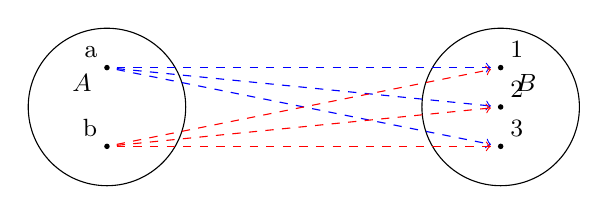
\begin{tikzpicture}[x=5mm,y=5mm,font=\small]

\def\firstcircle{(0,0) circle (2)}
\def\secondcircle{(10,0) circle (2)}

\draw \firstcircle node [above left=2]  {$A$};
\draw \secondcircle node [above right=2]  {$B$};

\fill (0,1) circle (1pt) node[above left] {a};
\fill (0,-1) circle (1pt) node[above left](b) {b};

\fill (10,1) circle (1pt) node[above right] {1};
\fill (10,0) circle (1pt) node[above right] {2};
\fill (10,-1) circle (1pt) node[above right] {3};

\node (a) at (0,1) {};
\node (b) at (0,-1) {};
\node (uno) at (10,1) {};
\node (due) at (10,0) {};
\node (tre) at (10,-1) {};
\begin{scope}[->,dashed]
\begin{scope}[blue]
\draw (a) -- (uno);
\draw (a) -- (due);
\draw (a) -- (tre);
\end{scope}
\begin{scope}[red]
\draw (b) -- (uno);
\draw (b) -- (due);
\draw (b) -- (tre);
\end{scope}
\end{scope}
\end{tikzpicture}

\end{center}

\paragraph{Tabella a doppia entrata}
Si costruisce una tabella nella quale si riportano gli elementi del
primo insieme sulla prima colonna e gli elementi del secondo insieme
sulla prima riga. Le caselle di incrocio rappresentano le coppie
ordinate del prodotto cartesiano.
\begin{center}
 % (c) 2012 Dimitrios Vrettos - d.vrettos@gmail.com
\begin{tikzpicture}[font=\small]

\matrix(m) [matrix of nodes, nodes={minimum size=7mm}]{
{}& 1 & 2 & 3\\
$a$ & $(a;1)$& $(a;2)$& $(a;3)$\\
$b$& $(b;1)$& $(b;2)$& $(b;3)$\\
};
\draw (m-2-1.north west)--(m-2-4.north east);
\draw (m-1-1.north east)--(m-3-1.south east);

\draw[decoration=brace,decorate] (m-1-2.north)--(m-1-4.north) node[above, midway] {$B$};
\draw[decoration={brace,mirror}, decorate] (m-2-1.west)--(m-3-1.west) node[left, midway] {$A$};

\end{tikzpicture}

\end{center}

\begin{wrapfloat}{figure}{r}{0pt}
 % (c) 2012 Dimitrios Vrettos - d.vrettos@gmail.com
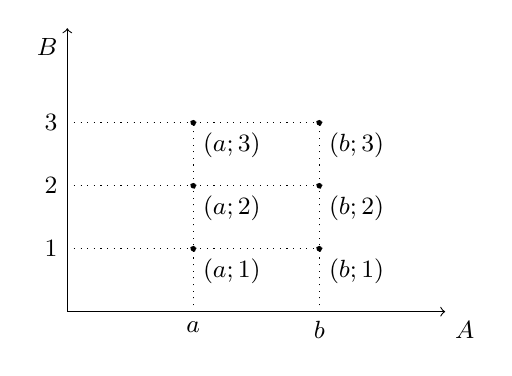
\begin{tikzpicture}[x=16mm, y=8mm,font=\small]
\draw[->] (0,0)--(3,0) node [below right]{$A$};
\draw[->] (0,0)--(0,4.5) node [below left]{$B$};

\begin{scope}[dotted]
\foreach \x in {1,2}
\foreach \y in {1,2,3}{
\draw (\x,0) -- (\x,\y);
\draw (0,\y) -- (\x,\y);
\draw[fill](\x,\y) circle (1pt);
}
\end{scope}

\begin{scope}[below right]
\node at (1,1) {$(a;1)$};
\node at (1,2) {$(a;2)$};
\node at (1,3) {$(a;3)$};
\node at (2,1) {$(b;1)$};
\node at (2,2) {$(b;2)$};
\node at (2,3) {$(b;3)$};
\end{scope}

\foreach \xi/\xitext in {1/$a$,2/$b$}
\node[below] at (\xi,0) {\xitext};

\foreach \yi/\yitext in {1/1,2/2,3/3}
\node[left] at (0,\yi) {\yitext};

\end{tikzpicture}

\end{wrapfloat}

\paragraph{Diagramma cartesiano}
Si tracciano due semirette una orizzontale e l'altra
verticale, orientate, perpendicolari, con l'origine
in comune. Si riportano gli elementi del primo insieme sulla semiretta
orizzontale e quelli del secondo su quella verticale. Tali semirette
vengono chiamate \emph{assi cartesiani}. Si tracciano prima le
parallele all'asse verticale dai punti
sull'asse orizzontale che rappresentano gli elementi
del primo insieme, poi le parallele all'asse
orizzontale dai punti sull'asse verticale; i punti di
intersezione rappresentano le coppie ordinate del prodotto
cartesiano.

\paragraph{Diagramma ad albero}
È un grafico formato da un nodo iniziale dal quale si ripartono alcuni
rami che a loro volta possono ramificarsi e così via fino a che nello
schema figurano tutte le possibili situazioni.

Si può raggiungere un particolare nodo solo muovendosi lungo i rami ed
il percorso che collega due nodi qualsiasi deve essere unico.

La rappresentazione mediante diagramma ad albero è vantaggiosa nel
caso si voglia fare il prodotto cartesiano tra più insiemi.
\begin{center}
% (c) 2012 Dimitrios Vrettos - d.vrettos@gmail.com
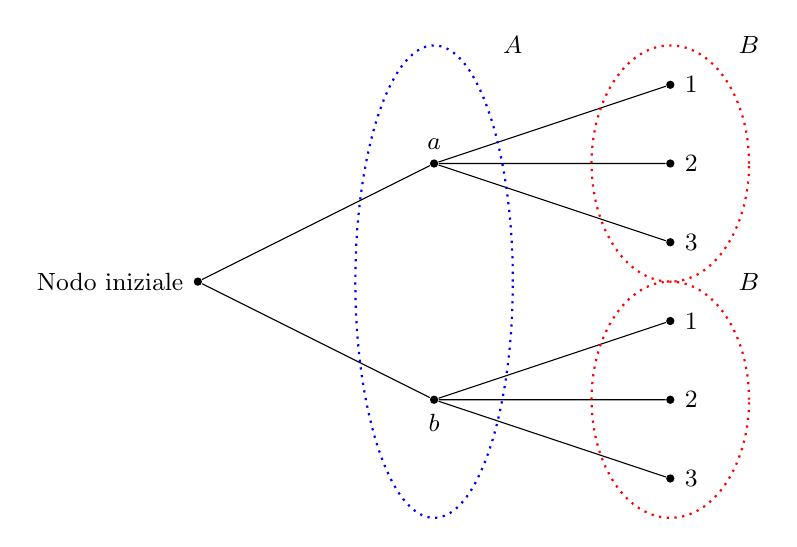
\begin{tikzpicture}[x=5mm, y=5mm,font=\small]
\tikzstyle{level 1}=[level distance=3cm, sibling distance=3cm]
\tikzstyle{level 2}=[level distance=3cm, sibling distance=1cm]
\tikzstyle{point} = [circle,minimum width=3pt,fill, inner sep=0pt]

\node[point, label=left:{Nodo iniziale}] (aer) at (0,0) {}[grow'=right]
child {node[point, label=above:{$a$}] {} 
child {node[point,label=right:{1}] {}}
child {node[point,label=right:{2}] {}}
child {node[point,label=right:{3}] {}}
}
child {node[point, label=below:{$b$}] {} 
child {node[point,label=right:{1}] {}}
child {node[point,label=right:{2}] {}}
child {node[point,label=right:{3}] {}}
} ;

\begin{scope}[dotted,thick]
\draw[blue] (6,0) ellipse (2 and 6)  (8,6)node [black] {$A$};
\draw[red] (12,3) ellipse (2 and 3) (14,6)node [black] {$B$};
\draw[red] (12,-3) ellipse (2 and 3)  (14,0)node [black] {$B$};

\end{scope}
\end{tikzpicture}

\end{center}

\begin{exrig}
 \begin{esempio}
 Una compagnia aerea deve organizzare delle rotte aeree per collegare fra 
 loro alcune città effettuando uno scalo in un'altra città. 
 Sia~$P=\{\text{Brindisi},\text{Bari},\text{Palermo}\}$ l'insieme delle città 
 di partenza, $S=\{\text{Roma},\text{Milano}\}$ l'insieme delle città di
 scalo e~$A=\{\text{Parigi},\text{Berlino},\text{Londra}\}$ l'insieme delle 
 città di arrivo. Per conoscere tutte le possibili rotte aeree dobbiamo
determinare il prodotto cartesiano tra i~3 insiemi~$P\times S\times A$.
Rappresentiamo~$P\times S\times A$ tramite un diagramma ad albero:

\begin{center}
% (c) 2012 Dimitrios Vrettos - d.vrettos@gmail.com
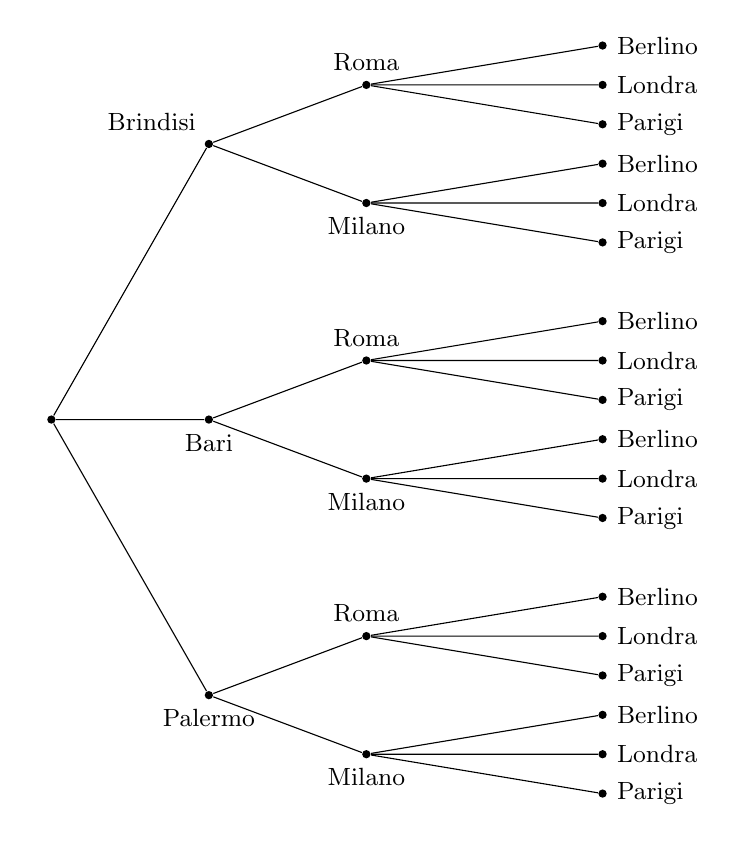
\begin{tikzpicture}[x=5mm, y=5mm,font=\small]
\tikzstyle{level 1}=[level distance=2cm, sibling distance=3.5cm]
\tikzstyle{level 2}=[level distance=2cm, sibling distance=1.5cm]
\tikzstyle{level 3}=[level distance=3cm, sibling distance=.5cm]
\tikzstyle{point} = [circle,minimum width=3pt,fill, inner sep=0pt]

\node[point, label=left:{}] (aer) at (0,0) {}[grow'=right]
  child {node[point, label=above left:{Brindisi}] {} 
    child {node[point,label=above:{Roma}] {}
      child {node[point, label=right:{Berlino}] {}}
      child {node[point, label=right:{Londra}] {}}
      child {node[point, label=right:{Parigi}] {}}
    }
    child {node[point,label=below:{Milano}] {}
      child {node[point, label=right:{Berlino}] {}}
      child {node[point, label=right:{Londra}] {}}
      child {node[point, label=right:{Parigi}] {}}}
    }
  child {node[point, label=below:{Bari}] {} 
    child {node[point,label=above:{Roma}] {}
      child {node[point, label=right:{Berlino}] {}}
      child {node[point, label=right:{Londra}] {}}
      child {node[point, label=right:{Parigi}] {}}}
    child {node[point,label=below:{Milano}] {}
      child {node[point, label=right:{Berlino}] {}}
      child {node[point, label=right:{Londra}] {}}
      child {node[point, label=right:{Parigi}] {}}}
    }
  child {node[point, label=below:{Palermo}] {} 
    child {node[point,label=above:{Roma}] {}
      child {node[point, label=right:{Berlino}] {}}
      child {node[point, label=right:{Londra}] {}}
      child {node[point, label=right:{Parigi}] {}}}
    child {node[point,label=below:{Milano}] {}
      child {node[point, label=right:{Berlino}] {}}
      child {node[point, label=right:{Londra}] {}}
      child {node[point, label=right:{Parigi}] {}}}
};
\end{tikzpicture}

\end{center}
 \end{esempio}
\end{exrig}

\section{I diagrammi di Eulero-Venn come modello di un problema}
\label{sec:insiemi_problemi}

Alcune volte, trovandoci di fronte a un problema, possiamo rappresentare
la situazione con diagrammi di Eulero-Venn, ciò agevola la
comprensione e facilita la risoluzione del problema. Attraverso alcuni
esempi mostreremo come usare la teoria degli insiemi per risolvere
problemi.

\begin{exrig}
 \begin{esempio}
Nel seguente diagramma di Eulero-Venn, l'insieme~$A$ rappresenta un gruppo di 
amici appassionati di ballo; gli insiemi~$T$, $R$,
$S$ rappresentano rispettivamente coloro che ballano il tango, la rumba, il 
samba; ogni puntino rappresenta uno degli amici.
\begin{multicols}{2}
Quanti sono gli amici appassionati di ballo?

Quanti tra loro ballano
\begin{enumeratea}
\item \emph{nessuno} dei balli indicati?
\item \emph{almeno uno} dei balli tango, samba, rumba?
\item \emph{almeno} il samba?
\item \emph{solo} la rumba?
\item la rumba \emph{e} il tango?
\item \emph{tutti} i balli indicati?
\end{enumeratea}
\begin{center}
 % (c) 2012 Dimitrios Vrettos - d.vrettos@gmail.com
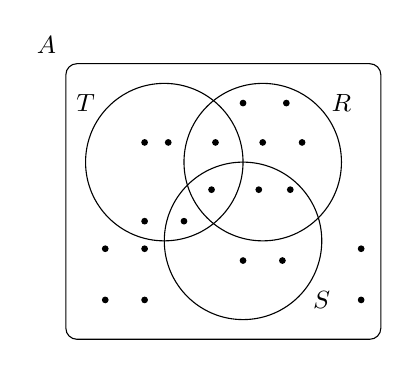
\begin{tikzpicture}[x=5mm, y=5mm,font=\small]

\draw[rounded corners] (0,0) rectangle (8,7) (0,7) node [above left]  {$A$};
\draw (2.5,4.5) circle (2) (.5,6)node {$T$};
\draw (5,4.5) circle (2) (7,6)node {$R$};
\draw (4.5,2.5) circle (2) (6.5,1)node {$S$};

\foreach \x in {2,2.6,3.8,5,6}
\draw[fill] (\x,5) circle (1pt);

\foreach \xi in {4.5,5.6}
\draw[fill] (\xi,6) circle (1pt);

\foreach \xii in {3.7,4.9,5.7}
\draw[fill] (\xii,3.8) circle (1pt);

\foreach \xiii in {2,3}
\draw[fill] (\xiii,3) circle (1pt);

\foreach \xiv in {4.5,5.5}
\draw[fill] (\xiv,2) circle (1pt);

\foreach \xv in {1,2,7.5}{
\draw[fill] (\xv,1) circle (1pt);
\draw[fill] (\xv,2.3) circle (1pt);
}
\end{tikzpicture}

\end{center}
\end{multicols}

Per rispondere alle domande dobbiamo contare gli elementi che formano 
determinati insiemi.

Quanti sono gli amici appassionati di ballo? Per rispondere a questa
domanda, contiamo tutti i puntini che compaiono nel disegno. Si ha 
$\card A=20$.

Rispondiamo ora alle altre domande.
\begin{enumeratea}
 \item Quanti tra loro ballano \emph{nessuno} dei balli indicati?
Chi non balla nessuno dei balli indicati sta nell'insieme~$A$, ma in nessuno 
degli insiemi $R$, $S$,$T$ quindi appartiene al complementare
di~$R\cup S\cup T$ rispetto all'insieme~$A$,
dunque~$\card (\overline{{R\cup S\cup T}})=6$.
 \item Quanti tra loro ballano \emph{almeno uno} dei balli tra tango, 
samba, rumba? Chi balla almeno uno di quei balli è rappresentato dagli elementi
dell'insieme~$R\cup S\cup T$, quindi~$\card(R\cup S\cup T)=14$.
 \item Quanti tra loro ballano \emph{almeno} il samba?
Gli amici che ballano almeno il samba sono nell'insieme
$S$, quindi~$\card S=6$.
 \item Quanti tra loro ballano \emph{solo} la rumba? Nell'insieme~$R$ 
sono rappresentati gli amici che ballano almeno il rumba, quindi dobbiamo 
togliere dall'insieme~$R$ gli elementi che stanno 
in $S$ o in~$T$:~$\card(R-(T\cup S))=4$.
 \item Quanti tra loro ballano la rumba \emph{e} il tango? 
Quelli che ballano sia la rumba che il tango sono gli elementi
dell'insieme intersezione~$R\cap T$, quindi~$\card(R\cap T)=2$.
 \item Quanti tra loro ballano \emph{tutti} i balli indicati? 
Quelli che ballano tutti e tre i balli indicati sono elementi
dell'insieme intersezione~$R\cap S\cap T$, quindi~$\card(R\cap S\cap T)=1$.
\end{enumeratea}

 \end{esempio}

 \begin{esempio}
 A settembre, per la festa delle contrade, a Lainate è arrivato un luna
park dove oltre ad una grande giostra era stato allestito un tiro a
segno con palline di gomma piuma, proprio per i bambini. Alcuni
bambini, accompagnati dalla loro maestra si sono recati al luna park: 7
sono stati sulla giostra, 3 sono stati sia sulla giostra che al tiro a
segno, 3 si sono divertiti solamente col tiro a segno e altri~2 sono
stati a guardare. Quanti bambini sono andati quel giorno al luna park?

\begin{multicols}{2}
Per risolvere il problema rappresentiamo con diagrammi di Eulero-Venn la 
situazione; indichiamo con~$B$ l'insieme dei bambini recatisi al luna park, 
con~$G$ l'insieme di quelli che sono stati sulla giostra e con~$T$ l'insieme
di quelli che hanno provato il tiro a segno.
Dall'enunciato sappiamo 
che~$\card(G)=7$, $\card(G\cap T)=3$, $\card(T-G)=3$ e~$card(B-(G\cup T))=2$.
\begin{center}
 % (c) 2012 Dimitrios Vrettos - d.vrettos@gmail.com
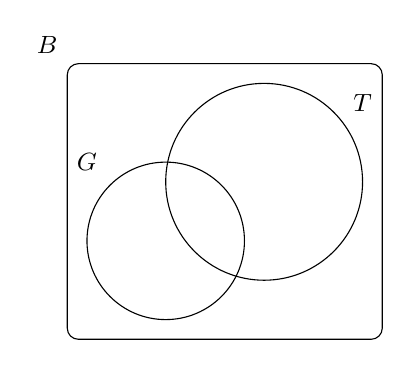
\begin{tikzpicture}[x=5mm, y=5mm,font=\small]

\draw[rounded corners] (0,0) rectangle (8,7) (0,7) node [above left]  {$B$};
\draw (2.5,2.5) circle (2) (.5,4.5)node {$G$};
\draw (5,4) circle (2.5) (7.5,6)node {$T$};

\end{tikzpicture}

\end{center}
\end{multicols}

Completa la rappresentazione segnando i bambini con dei puntini e rispondi 
al quesito.
\end{esempio}

\begin{esempio}
Alla palestra Anni Verdi, il giovedì, si tengono due allenamenti di pallavolo 
e calcio dalle~17.00 alle~18.30. Frequentano il corso di
pallavolo~15 persone e sono~28 quelli che frequentano l'allenamento di calcio. 
Quante persone frequentano pallavolo o calcio in questo orario?

\paragraph{Dati} $P=\{\text{iscritti a pallavolo}\}$, $C=\{\text{iscritti a 
calcio}\}$, $\card(P)=15$, $\card(C)=28$.

\paragraph{Obiettivo} Il problema chiede di determinare la cardinalità 
di~$P\cup C$.

%\begin{multicols}{2}
\paragraph{Soluzione} Osserviamo che non ci sono persone che frequentano sia
l'uno che l'altro sport essendo gli allenamenti nello stesso orario; gli 
insiemi~$P$ e~$C$ sono disgiunti:~$P\cap C=\emptyset $. 
Quindi:~$\card(P\cup C)=\card(P)+\card(C)=15+28=43$.

% \begin{center}
% % (c) 2012 Dimitrios Vrettos - d.vrettos@gmail.com
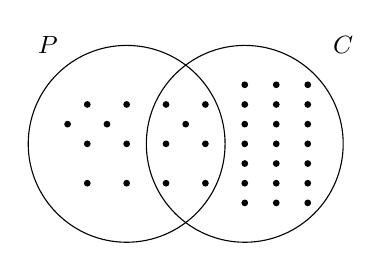
\begin{tikzpicture}[x=5mm, y=5mm,font=\small]

\draw (2,0) circle (2.5) (0,2.5)node {$P$};
\draw (5,0) circle (2.5) (7.5,2.5)node {$C$};

\foreach \x in {1,2,3,4}
\foreach \y in {-1,0,1}
\draw[fill] (\x,\y) circle (1pt);

\foreach \z in {.5,1.5,3.5}
\draw[fill] (\z,.5) circle (1pt);

\foreach \i in {5,5.8,6.6}
\foreach \j in {1.5,1,.5,0,-.5,-1,-1.5}
\draw[fill] (\i,\j) circle (1pt); 
\end{tikzpicture}

% \end{center}
%\end{multicols}
\end{esempio}
\begin{esempio}
\begin{multicols}{2}
 Alla palestra Anni Verdi, il lunedì si tengono allenamenti di pallavolo, 
 dalle~17.00 alle~18.30 e dalle~19.00 alle~20.30 gli allenamenti di calcio. 
 Quelli che frequentano la pallavolo sono~15, quelli che frequentano il calcio 
 sono~28, però ce ne sono~7 di loro che fanno entrambi gli allenamenti. 
 Quanti sono gli sportivi che si allenano il lunedì?
\begin{center}
 % (c) 2012 Dimitrios Vrettos - d.vrettos@gmail.com
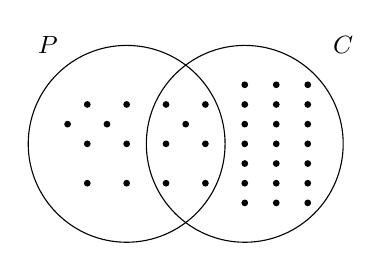
\begin{tikzpicture}[x=5mm, y=5mm,font=\small]

\draw (2,0) circle (2.5) (0,2.5)node {$P$};
\draw (5,0) circle (2.5) (7.5,2.5)node {$C$};

\foreach \x in {1,2,3,4}
\foreach \y in {-1,0,1}
\draw[fill] (\x,\y) circle (1pt);

\foreach \z in {.5,1.5,3.5}
\draw[fill] (\z,.5) circle (1pt);

\foreach \i in {5,5.8,6.6}
\foreach \j in {1.5,1,.5,0,-.5,-1,-1.5}
\draw[fill] (\i,\j) circle (1pt); 
\end{tikzpicture}

 \end{center}
\end{multicols}

\paragraph{Dati} $P=\{\text{iscritti a pallavolo}\}$, 
 $C=\{\text{iscritti a calcio}\}$, $\card(P)=15$, 
 $\card(C)=28$ e~$\card(P\cap C)=7$.
 
\paragraph{Obiettivo} Il problema chiede di determinare la cardinalità 
di~$P\cup C$.

\paragraph{Soluzione} 
 $\card(P\cup C)=\card(P)+\card(C)-\card(P\cap C)=15+28-7=36$.

Generalizzando possiamo affermare \ che dati due insiemi finiti~$A$ e~$B$ 
la cardinalità dell'insieme~$A\cup B$ è data dalla seguente formula:
$\card(A\cup B)=\card(A)+\card(B)-\card(A\cap B)$.
\end{esempio}

\begin{esempio}
 A scuola si sono aperti i corsi di lingue. Della classe di Piero, che è 
 composta da~28 ragazzi,~17 frequentano il corso di inglese,~12
quello di francese,~5 di loro frequentano sia il corso di inglese, sia quello 
di francese. Quanti sono i ragazzi della classe di Piero che non
frequentano alcun corso di lingue?

Rappresentiamo la situazione con un diagramma di Eulero-Venn.
\begin{multicols}{2}
L'insieme universo è costituito dai~28 ragazzi che
compongono la classe. I ragazzi che frequentano almeno un corso \emph{non} 
sono~$17+12=29$, perché ce ne sono~5 che frequentano entrambi i corsi e
vengono conteggiati due volte. Quindi i ragazzi che frequentano almeno un 
corso sono~$17+12-5=24$. Di conseguenza quelli che non frequentano
nessun corso sono~$28-24=4$.
\begin{center}
 % (c) 2012 Dimitrios Vrettos - d.vrettos@gmail.com
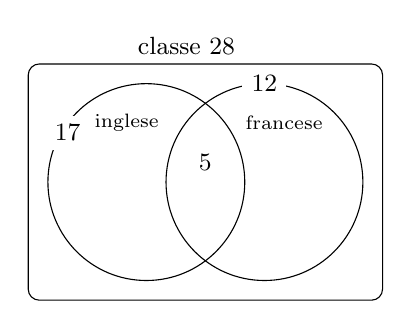
\begin{tikzpicture}[x=5mm, y=5mm,font=\small]

\draw[rounded corners] (-1,-3) rectangle (8,3) (4.5,3)node[above, anchor=south east] {classe 28};
\draw (2,0) circle (2.5);
\draw (5,0) circle (2.5);

\begin{scope}[font=\scriptsize]
\node at (1.5,1.5) {inglese};
\node at (5.5,1.5) {francese};
\end{scope}

\node at (3.5,.5) {5};
\node[fill=white] at (0,1.25) {17};
\node[fill=white] at (5,2.5) {12};
\end{tikzpicture}

\end{center}
\end{multicols}
\end{esempio}

\begin{esempio}
 Il professore di matematica di Piero è piuttosto severo; nella sua classe, 
 di~28 alunni, ha messo solo~6 sufficienze allo scritto e solo~8 all'orale. 
 I ragazzi che sono risultati insufficienti sia allo scritto sia 
all'orale sono stati~18. 
Quanti sono i ragazzi che hanno avuto una votazione sufficiente sia allo 
scritto che all'orale?

Rappresentiamo la situazione con un diagramma di Eulero-Venn.
\begin{multicols}{2}
$C$ è l'insieme degli alunni della classe di Piero, è costituito da~28 
elementi. $S$ è l'insieme dei ragazzi sufficienti allo scritto, 
è costituito da~6 alunni. $O$ è l'insieme dei ragazzi che sono sufficienti
all'orale, è costituito da~8 elementi.

Gli elementi di~$\overline{{S\cup O}}$ sono~18, cioè i ragazzi che
non sono sufficienti né allo scritto, né all'orale.
\begin{center}
 % (c) 2012 Dimitrios Vrettos - d.vrettos@gmail.com
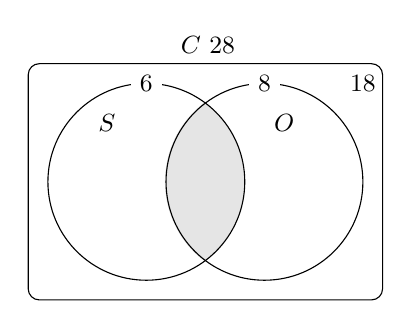
\begin{tikzpicture}[x=5mm, y=5mm,font=\small,filled/.style={fill=circle area, draw=circle edge, thick}]
\def\firstcircle {(2,0) circle (2.5)}
\def\secondcircle{(5,0) circle (2.5)}

\definecolor{circle edge}{gray}{0.9}
\definecolor{circle area}{gray}{0.9}
\draw[rounded corners] (-1,-3) rectangle (8,3) (4.5,3)node[above, anchor=south east] {$C$ 28};
\begin{scope}
\clip \firstcircle;
\fill[filled] \secondcircle;
\end{scope}
\draw\firstcircle;
\draw \secondcircle;

\node at (1,1.5) {$S$};
\node at (5.5,1.5) {$O$};
\node  at (7.5,2.5) {18};

\node[fill=white] at (2,2.5) {6};
\node[fill=white] at (5,2.5) {8};

\end{tikzpicture}

\end{center}
\end{multicols}

L'insieme~$S\cup O$ è quindi costituito da~$28-18=10$ elementi.

Ricordiamo che
\begin{align*}
 &\card(S\cup O)=\card(S)+\card(O)-\card(S\cap O)\\
 \Rightarrow &\card(S\cap O)=\card(S)+\card(O)-\card(S\cup O)\\
 \Rightarrow &\card(S\cap O)=6+8-10=4.
\end{align*}
In conclusione i ragazzi sufficienti allo scritto e all'orale sono~4.
\end{esempio}
\end{exrig}

% \ovalbox{\risolvii \ref{ese:7.25}, \ref{ese:7.26}, \ref{ese:7.27}, \ref{ese:7.28}, \ref{ese:7.29}, \ref{ese:7.30}, \ref{ese:7.31}, \ref{ese:7.32}, \ref{ese:7.33}, \ref{ese:7.34},
% \ref{ese:7.35}, \ref{ese:7.36}, \ref{ese:7.37}}
% 
% \vspazio\ovalbox{\ref{ese:7.38}}

